%%%%%%%%%%%%%%%%%%%%%%%%%%%%%%%%%%%%%%%%%%%%%%%%%%%%%%%%%%%%%%%%%%%%%%%%%%

% abnTeX2: Modelo de Trabalho Acadêmico em conformidade com
% as normas da ABNT

%%%%%%%%%%%%%%%%%%%%%%%%%%%%%%%%%%%%%%%%%%%%%%%%%%%%%%%%%%%%%%%%%%%%%%%%%%

\documentclass[english,
               brazil,
               bsc] %Opções bsc (TCC) e msc (Mestrado)
               {dcomp-abntex2}


%%%%%%%%%%%%%%%%%%%%%%%%%%%%%%%%%%%%%%%%%%%%%%%%%%%%%%%%%%%%%%%%%%%%%%%%%%
% Área para adição de pacotes extras
%%%%%%%%%%%%%%%%%%%%%%%%%%%%%%%%%%%%%%%%%%%%%%%%%%%%%%%%%%%%%%%%%%%%%%%%%%

\usepackage{lipsum} %Retirar para a versão final do documento

%Utilize aqui seu pacote preferido para algoritmos
\usepackage[linesnumbered]{algorithm2e}

%%%%%%%%%%%%%%%%%%%%%%%%%%%%%%%%%%%%%%%%%%%%%%%%%%%%%%%%%%%%%%%%%%%%%%%%%%

%Compila o indice
\makeindex

\begin{document}

% Seleciona o idioma do documento (conforme pacotes do babel)
\selectlanguage{brazil}

% Retira espaço extra obsoleto entre as frases.
\frenchspacing

%%%%%%%%%%%%%%%%%%%%%%%%%%%%%%%%%%%%%%%%%%%%%%%%%%%%%%%%%%%%%%%%%%%%%%%%%%
% ELEMENTOS PRÉ-TEXTUAIS
%%%%%%%%%%%%%%%%%%%%%%%%%%%%%%%%%%%%%%%%%%%%%%%%%%%%%%%%%%%%%%%%%%%%%%%%%%

\pretextual

\titulo{AtalaIA: Compressão de modelos de detecção de velocidade de veículos}
\autor{Luan Fabrício de Carvalho Lima Leite}
\orientador{Leonardo Nogueira Matos}
\coorientador{Rafael Andrade da Silva}
\curso{Ciência da Computação}

\inserirInformacoesPDF

\imprimircapa
\imprimirfolhaderosto*

\begin{dedicatoria}
   \vspace*{\fill}
   \centering
   \noindent
   \textit{Dedico este trabalho a minha família, amigos, professores e todos que de alguma forma me ajudaram a chegar até aqui.}
   \vspace*{\fill}
\end{dedicatoria}
% ---

\begin{agradecimentos}


\end{agradecimentos}
% ---

\begin{epigrafe}[]
    \vspace*{\fill}
	\begin{flushright}

		\textit{I may not have gone where I intended to go, \\
			but I think I have ended up where I needed to be. \\
			(Dougas Adams)}
	\end{flushright}
\end{epigrafe}
% ---

% resumo em português
\setlength{\absparsep}{18pt} % ajusta o espaçamento dos parágrafos do resumo
\begin{resumo}

Redes Neurais Convolucionais estão ficando cada vez mais populares para solução de diversos desafios, sendo um deles
o de reconhecimento facial, que é uma das tarefas onde essa abordagem já supera o ser humano.
Entretanto, esse método costuma exigir um alto poder de processamento e quantidade de memória, o que acaba
limitando o seu uso em casos de computação de borda com dispositivos embarcados.
Este trabalho tem como foco tratar esse problema, comprimindo um modelo de reconhecimento facial para que ele seja
embarcado e consiga realizar operações na borda, mantendo a acurácia alta e tempo de resposta baixo.
Para que esse objetivo seja cumprido, será necessário utilizar um modelo como base, para que ele seja comprimido e
avaliado, onde ele será escolhido a partir da comparação de soluções já existentes e utilizadas.
O modelo embarcado será avaliado com base em métricas como acurácia, F1 score, latência e ocupação de memória e
comparado a outras soluções existentes.

 \textbf{Palavras-chave}: CNN, Compressão de modelos, Visão computacional, Sistemas embarcados, Computação em borda,
 Reconhecimento facial
\end{resumo}

% resumo em inglês
\setlength{\absparsep}{18pt} % ajusta o espaçamento dos parágrafos do resumo
\begin{resumo}[Abstract]
 \begin{otherlanguage*}{english}
   Convolutional Neural Networks are becoming increasingly popular for solving various challenges, one of them being
   facial recognition, which is one of the tasks that this approach overcomes humans.
   However, this method usually requires a high computational power and amount of memory, which ends up limiting its
   use case in edge computing for embedded devices.
   This work focuses on addressing this issue, compressing a facial recognition model so that it is embedded and can
   perform operations at the edge, maintaining high accuracy and low response time.
   For this objective to be achieved, it will be necessary to use a model as a basis, so that it can be compressed and
   evaluated, where it will be chosen based on the comparison of the existing and used
   solutions.
   % TODO: traduzir essa parte
   To finish, this model will be embedded to perform operations on edge, both inference and processing on the device,
   from there, its effectiveness will be measured and compared with other solutions already created.

   \vspace{\onelineskip}

   \noindent
   \textbf{Keywords}: CNN. Model compression. Computer Vision. Embedded systems. Edge computing. Facial recognition.
 \end{otherlanguage*}
\end{resumo}



\mostrarlistadeILUSTRACOES
\mostrarlistadeQUADROS
\mostrarlistadeTABELAS
\mostrarlistadeCODIGOS
\mostrarlistadeALGORITMOS

% Lista de abreviaturas e siglas

\begin{siglas}
	\item[ABNT]{Associação Brasileira de Normas Técnicas}
	\item[abnTeX]{ABsurdas Normas para TeX}
  	\item[DCOMP]{Departamento de Computação}
	\item[UFS]{Universidade Federal de Sergipe}
	\item[ANN]{Rede Neural Artificial ou \textit{Artificial Neural network}}
	\item[CNN]{Rede Neural Convolucional ou \textit{Convolutional Neural Network}}
	\item[KB]{Kilobytes}
	\item[MB]{Megabytes}
	\item[API]{Interface de Programação de Aplicações ou \textit{Application Program Interface}}
	\item[IoT]{Internet das Coisas ou \textit{Internet of Things}}
\end{siglas}

% ---
% inserir lista de símbolos
% ---

\begin{simbolos}
  \item[$ \alpha $] Letra grega alfa
  \item[$ \Gamma $] Letra grega Gama
  \item[$ \Lambda $] Lambda
  \item[$ \zeta $] Letra grega minúscula zeta
  \item[$ \in $] Pertence
\end{simbolos}
% ---


\mostrarSUMARIO

%%%%%%%%%%%%%%%%%%%%%%%%%%%%%%%%%%%%%%%%%%%%%%%%%%%%%%%%%%%%%%%%%%%%%%%%%%
% ELEMENTOS TEXTUAIS
%%%%%%%%%%%%%%%%%%%%%%%%%%%%%%%%%%%%%%%%%%%%%%%%%%%%%%%%%%%%%%%%%%%%%%%%%%

\textual
\chapter{Introdução}

% TODO: Melhorar e aprofundar sobre ANN
Redes Neurais Artificiais, ou \textit{Artificial Neural Network} (ANN), são ferramentas poderosas para auxiliar a
sociedade.
Podendo ser utilizadas em diversas tarefas, como reconhecimento facial, onde a rede é treinada para realizar a
classificação da face da pessoa, permitindo que ela seja usada em várias áreas diferentes, indo de entretenimento até
segurança.

\section{Motivação}
% TODO: Talvez seja interessante rescrever para exaltar que o
% motivo foi o artigo
O uso de Redes Neurais Artificiais vem crescendo bastante no ramo de computação visual, principalmente desde 2012,
quando Redes Neurais Convolucionais ou \textit{Convolutional Neural Networks} (CNN) começaram a ser utilizadas para
classificação de imagens \cite{alexnet}.
Um dos usos desse tipo de rede é na detecção de face, que é muito relevante para a área de segurança e
vigilância, onde o modelo pode fazer a detecção do rosto de uma pessoa, abrir uma porta ou enviar uma notificação
para algum segurança.
Porém, essa abordagem necessita de uma quantidade elevada de poder computacional, tornando inviável que tal tipo de
produto seja embarcado e mantenha um baixo tempo de resposta, o que pode atrapalhar a experiência do usuário, ou
reduzir a efetividade da ação que será tomada.

Um dos principais problemas das Redes Neurais Profundas, como CNN, é que elas necessitam de um alto processamento e uso
de memória, o que acaba dificultando a sua execução em dispositivos com poder computacional e memória limitados (como os dispositivos embarcados).
Porém, existem técnicas que podem ser aplicadas para reduzir o poder computacional necessário, como o uso de
destilação de conhecimento \cite{hinton2015distilling}, poda e quantização.
Possibilitando a implantação do modelo em sistemas embarcados na borda, de forma que a latência do dispositivo seja
baixa.

\section{Objetivos}

O objetivo deste trabalho é comprimir uma Rede Neural Convolucional, permitindo que ela realize o reconhecimento
facial em microcontroladores, na borda.
Nele também serão tratadas formas de comprimir e otimizar o modelo, para que a sua versão final consiga ser embarcada
em um dispositivo com hardware limitado, mantendo acurácia alta e baixa latência.

\subsection{Objetivo específicos}
O trabalho estará completo se os seguintes objetivos forem alcançados:

\begin{itemize}
	% TODO: Reescrever, deixando claro que o objetivo é embarcar o modelo.
	% Deixar claro que é necessário que o modelo comprimido também tenha uma alta acurácia, F1-score etc.
	% Deixar claro que é necessário que o modelo comprimido não utilize poucos recursos computacionais
	%	(armazenamento, memória e uso de cpu) e que a latência também seja baixa.
	\item Aplicar técnicas de compressão e otimização em um modelo, assim reduzindo o uso de CPU e memória,
		o permitindo que seja embarcado.
	% TODO: Rever
	\item Validar performace do modelo, para garantir que a acurácia e F1-score do modelo seja mantida.
	\item Embarcar o modelo comprimido de forma que ele consiga realizar operações na borda, mantendo acurácia
		alta e baixa latência.
\end{itemize}

\section{Metodologia}
Para atingir o objetivo do estudo, foi necessário dividir o processo em algumas etapas, cada uma sendo
essencial para que o objetivo do trabalho fosse atingido. Sendo elas:

\begin{enumerate}
	\item \textbf{Levantamento do estado da arte:}

		Nessa etapa, são selecionados artigos que possuem o objetivo similar ao deste artigo,
		com base nesses artigos serão testadas novas técnicas para compressão de modelos.

	\item \textbf{Reprodução do estado da arte:}
		% TODO: Explicar melhor o que foi feito nesta etapa.
		% Verificar se ela irá aparecer na etapa final do trabalho.
		% TODO: Revisar

	\begin{enumerate}
		\item \textbf{Seleção de base e treino de modelos:}

			Nesta etapa, uma base de dados é selecionada e a partir dela serão desenvolvidos modelos,
			com o objetivo de atingir uma alta acurácia, sem sofrer \textit{overfitting}.

		\item \textbf{Aplicação de técnicas de compressão para Modelos:}

			Após definir e treinar os modelos, serão aplicadas técnicas de compressão, tendo como
			objetivo ter uma acurácia parecida com a do modelo original. Onde as técnicas aplicadas
			foram: poda, quantização e destilação de conhecimento.

		\item \textbf{Avaliação do desempenho:}

			Depois de treinar e aplicar técnicas de compressão, os dados dos modelos serão coletados e
			avaliados. Para realizar essa avaliação, será necessário utilizar um conjunto de testes.

		\item \textbf{Análise e comparação dos resultados:}

			Para finalizar, os dados dos modelos serão comparados e analisados. Com o objetivo de
			identificar o melhor modelo e descobrir quais foram os motivos para que esse modelo tenha se
			saído melhor, mesmo após a aplicação de compressão. Nesta etapa as métricas de acurácia e
			tamanho do modelo são avaliadas.
	\end{enumerate}

	\item \textbf{Escolha do modelo para reconhecimento facial:}

		Nesta etapa serão avaliados os modelos com base em métricas como acurácia, F1 score, latência e ocupação de
		memória. Após a avaliação será escolhido um modelo que servirá como base nas próximas etapas.

	\item \textbf{Compressão e implantação do modelo em hardware limitado:}

		Depois de escolher um modelo de reconhecimento facial, ele será comprimido de forma que possa ser executado
		em sistemas embarcados, mantendo a acurácia alta e latência baixa.

	\item \textbf{Desenvolvimento do estudo de caso:}

		Com o modelo final comprimido ao ponto de ser implantado em um sistema embarcado, será desenvolvida uma aplicação 	 	 que servirá como experimento para avaliar a eficácia do modelo dentro de dispositivos com hardware limitado.

\end{enumerate}

As etapas 3, 4 e 5 serão realizadas no Trabalho de Conclusão de Curso 2.

\section{Estrutura do documento}
Este documento foi dividido em capítulos, onde cada um apresenta uma proposta diferente:
\begin{itemize}
	\item Capítulo 2 - \textbf{Conceitos Básicos}: Apresenta os tópicos principais para o entendimento
		do trabalho.
	\item Capítulo 3 - \textbf{Trabalhos Relacionados}: Apresenta uma revisão dos trabalhos
		relacionados ao tema do trabalho.
	\item Capítulo 4 - \textbf{Resultados Preliminares}: Apresenta os resultados preliminares dos
		experimentos realizados durante o trabalho.
	\item Capítulo 5 - \textbf{Planos de continuidade}: Contém o planejamento da continuidade do
		Trabalho de Conclusão 2.
\end{itemize}

\chapter{Conceitos básicos}\label{cap_conceitos}

\chapterprecis{Isto é uma sinopse de capítulo. A ABNT não traz nenhuma
normatização a respeito desse tipo de resumo, que é mais comum em romances
e livros técnicos.}\index{sinopse de capítulo}

\section{Redes Neurais Artificiais}\label{cap_conceitos_ann}
% ---
Redes Neurais Artificiais (ANNs), são neurônios interconectados que realizam um processamento simples. Dentro dessa
estrutura cada neurônio reforça ou enfraquece a conexão com um dos neurônio da coluna anterior, assim replicando
o processo de aprendizagem do cérebro humano. A \autoref{cap_conceitos_ann_exemplo_ann} exemplifica uma ANN bem
simples.

\begin{figure}[htb]
	\caption {\label{cap_conceitos_ann_exemplo_ann}Exemplo de uma ANN}
	\begin{center}
		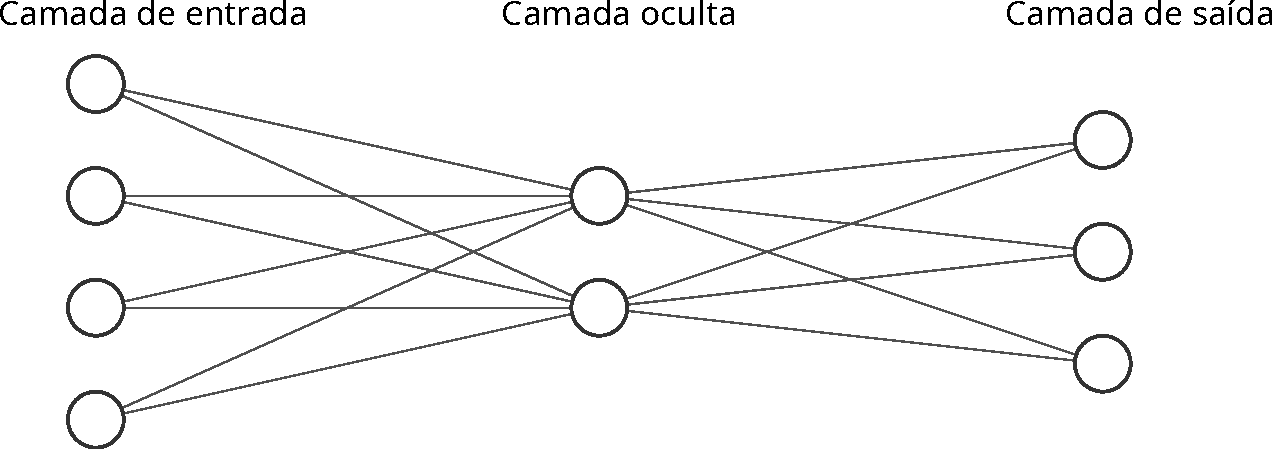
\includegraphics[scale=0.5]{Imagens/exemplo_nn}
	\end{center}
	\legend {Fonte: Autor}
\end{figure}

O neurônio é uma parte fundamental de uma ANN, nele que o aprendizado é armazenado através do reforço de conexões com
outros neurônio. Esse reforço é o peso da conexão, ele é multiplicado pela entrada e somado com os outros valores,
como é demonstrado na equação \ref{eq_neuronio} (onde $x$ é um vetor com os valores de entrada do neurônio e $w$
é um vetor com os pesos de cada entrada). Depois disso os valores passam por uma função de ativação $g(x)$ (\ref
{eq_ativacao}), que é responsável por "tratar" esses dados de saída antes que eles sejam passados para próxima etapa.

\begin{equation}\label{eq_neuronio}
u = \sum x_i w_i
\end{equation}
\begin{equation}\label{eq_ativacao}
y = g(u + b)
\end{equation}

\begin{figure}[htb]
	\caption {\label{cap_conceitos_ex_neuronio} Exemplo de um neurônio artificial}
	\begin{center}
		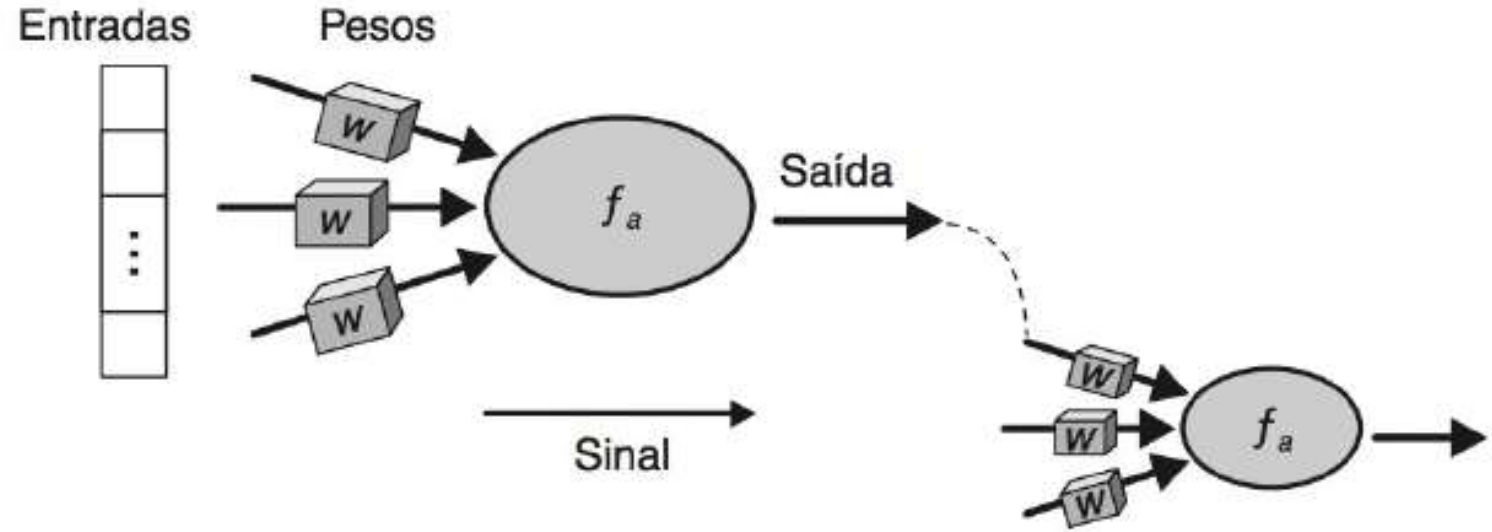
\includegraphics[scale=0.3]{Imagens/exemplo_neuronio_artificial}
	\end{center}
	\legend{Fonte: \cite{ml-faceli}}
\end{figure}

\section{Redes Neurais Convolucionais}\label{cap_conceitos_cnn}
% ---
Redes Neurais Convolucionais (CNNs) são Redes Neurais Artificiais (ANN)
que utilizam a operação de convolução para o processamento e análise de dados no formato de \textit{grid}(grade).
Por exemplo, uma série temporal que pode ser representada no formato de \textit{grid} 1-D,
ou uma imagem, que pode ser representada no formato 2-D. \cite{Goodfellow-et-al-2016}
Onde, LeNet \cite{lenet}, Residual Network (ResNet) \cite{resnet} e AlexNet \cite{alexnet} são alguns exemplos de CNNs
famosas.
% (TODO: Adicionar exemplos)

A arquitetura de uma CNN é composta por camadas convolucionais (\ref{cap_conceitos_cnn_conv}),
\textit{pooling} (\ref{cap_conceitos_cnn_pooling}) e totalmente conectadas (\ref{cap_conceitos_cnn_totalmente}),
como podemos ver na \autoref{exemplo_lenet}.

\begin{figure}[htb]
	\caption {\label{exemplo_lenet} Arquitetura da LeNet}
	\begin{center}
		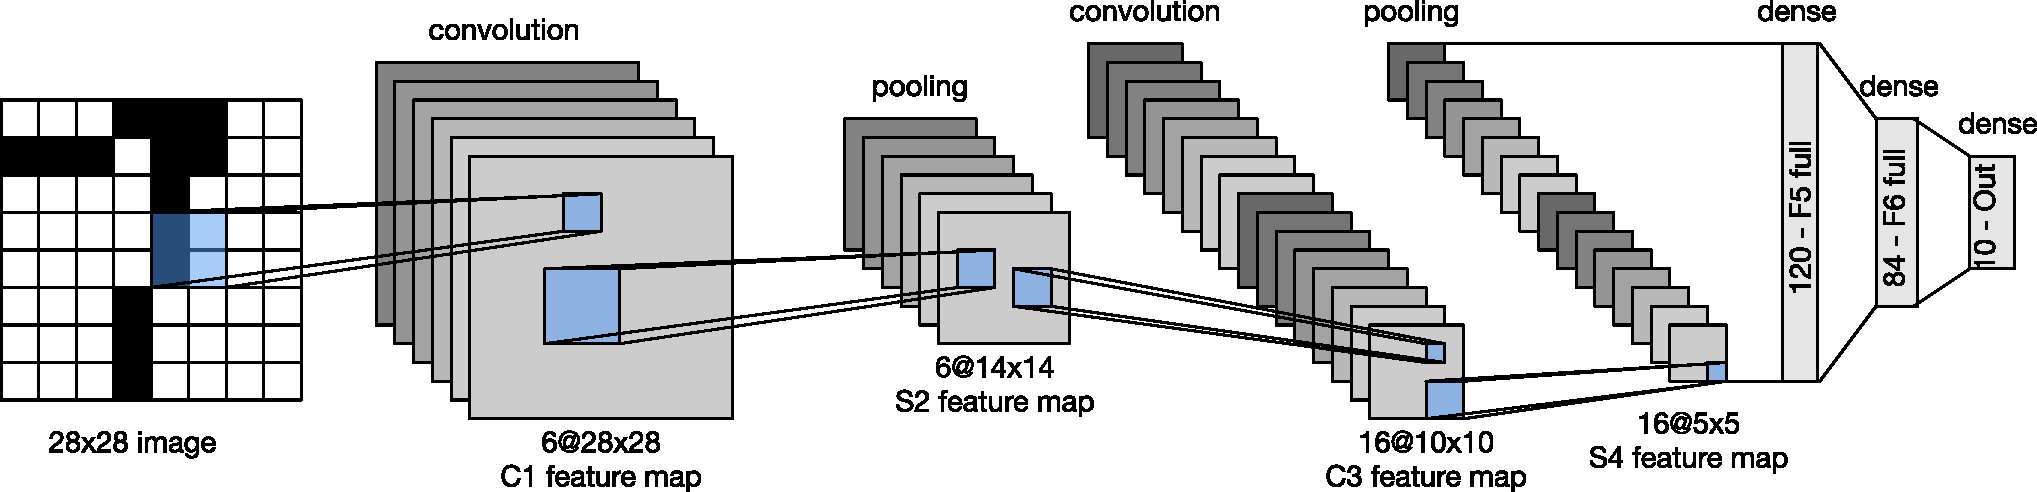
\includegraphics[scale=0.5]{Imagens/lenet}
	\end{center}
	\legend{Fonte: \cite{zhang2023dive}}
\end{figure}

\subsection{Camada de Convolução}\label{cap_conceitos_cnn_conv}
Nessa camada são aplicados filtros (matriz de pesos) nos dados de entrada,
onde esses filtros deslizam cada célula da imagem executando operações de multiplicação e soma
em cada elemento da matriz de entrada, com o objetivo de gerar um mapa de características (\textit{feature map}).
O objetivo desses filtros é realçar as características dos dados de entrada, como curvas, linhas e outros padrões.
% (TODO: Adicionar figuras, referências e detalhar mais)

\subsection{Camada de \textit{pooling}}\label{cap_conceitos_cnn_pooling}
% ---
A abordagem da camada de \textit{pooling} é um pouco parecida com a camada de convolução,
uma matriz desliza pelas células da imagem, salvando apenas o maior valor dessa área na matriz de saída.
A partir disso, a camada consegue reduzir o tamanho da matriz de entrada, fazendo com que o poder computacional
necessário seja reduzido, junto com o uso de memória.
(TODO: Adicionar figuras, referências e detalhar mais)

\subsection{Camada totalmente conectada}\label{cap_conceitos_cnn_totalmente}
% ---
A camada totalmente conectada (\textit{fully connected layer}) é a camada final de uma CNN.
Depois das camadas anteriores extraírem as características da imagem, a camada totalmente
conectada as interpreta e gerar uma resposta.
(TODO: Revisar texto)

\section{\textit{Data augmentation}}
% ---
CNNs tem um ótimo desempenho em tarefas de visão computacional. Entretanto esse tipo de rede neural precisa de uma
grande quantidade dados para não sofrer de \textit{overfitting} (superajuste). \cite{shorten2019survey}
Esse é o objetivo do \textit{data augmentation} (aumento de dados), gerar mais dados a partir de um conjunto de dados
que já existe, aplicando algumas transformações geométricas ou espaciais, ou realizam injeção de ruído nas imagens
originais.

% TODO: Adicionar exemplo de data augmentation.

\section{Transferência de conhecimento}\label{conceitos_transferencia}
% ---
Transferência de conhecimento consiste em usar um modelo pré-treinado em uma base de dados específica e aproveitar
o conhecimento adquirido durante esse treinamento para um novo conjunto de dados.
É necessário que o problema do \textit{dataset} (conjunto de dados) atual seja um subconjunto do \textit{dataset}
que foi usado para treinar o modelo base.

Para realizar a transferência de conhecimento é necessário adaptar a camada de entrada e de saída
(totalmente conectada) do modelo base, para que ocorra um pré-processamento dos dados de entrada
(antes deles serem passados para o modelo base), além disso é necessário definir e treinar a camada totalmente
conectada com o \textit{dataset} do problema.

\section{Métodos de compressão para Redes Neurais}
ANNs são utilizadas em várias aplicações, demonstrando habilidades extraordinárias no campo de visão computacional.
No entanto, redes com arquiteturas complexas são um desafio para a implantação em tempo real e necessitam de uma
grande quantidade de energia e poder computacional \cite{LIANG2021370}.
Por causa disso foram desenvolvidos métodos para reduzir o tamanho dessas redes, as tornando mais eficiente.
Nesse trabalho os métodos de poda (\ref{poda}), quantização (\ref{quantizacao}) e destilamento do conhecimento
(\ref{conceitos_destilamento}) serão usados.

\subsection{\textit{Pruning}(Poda)}\label{poda}
A poda de redes neurais tem como objetivo principal remover pesos ou neurônios que são
redundantes ou irrelevantes para o problema, além disso reduz o \textit{overfitting}(superajuste).
(TODO: escrever sobre poda de redes neurais)

% Redes neurais costumam usar muito recurso computacional e otimizar o uso dos recursos é muito importante para
% aplicações de grande escala. A poda de redes neurais tem como objetivo principal remover pesos ou neurônios que são
% redundantes ou irrelevantes para o problema, além disso reduz o \textit{overfitting}(superajuste).

\subsection{Quantização}\label{quantizacao}

% Quantization reduces computations by reducing the precision of the datatype. Weights, biases, and activations
% may be quantized typically to 8-bit integers although lower bit width implementations are also discussed including
% binary neural networks. Both pruning and quantization can be used independently or combined.

Quantização reduz a computação diminuindo a precisão dos tipos de dados. Pesos, \textit{bias} (vieses) e ativações
geralmente devem ser quantizadas para inteiros de 8 bit, embora implementações menores que 8 bit sejam discutidas
incluindo redes neurais binárias. \cite{LIANG2021370}

% (TODO: Escrever sobre quantização)

\subsection{Destilamento de conhecimento (Professor-Aluno)}\label{conceitos_destilamento}

Destilamento de conhecimento ou \textit{knowledge distillation} \cite{hinton2015distilling}, é uma técnica que tem
como objetivo treinar um modelo Aluno (menor e sem pré-treinamento) com um modelo Professor
(maior e com pré-treinamento). Ela é amplamente utilizada para as áreas de visão computacional e linguagem natural,
e tem como objetivo reduzir o tamanho do modelo final (Aluno).

Para transferir o conhecimento do modelo Professor para o Aluno, a técnica utiliza os \textit{logits} (entrada da
função de ativação final \textit{softmax}) no lugar da classe prevista. Além disso, são utilizado os
\textit{soft targets} (probabilidades das classes previstas pelo modelo Professor) junto com os
\textit{hard targets} (classe esperada). Então, o Aluno é treinado com uma porcentagem $\alpha$ do erro com o
\textit{hard target} e $\alpha - 1$ do erro com \textit{soft target}, assim é calculado o erro do aluno.

% NOTE: Talvez detalhar a temperatura?

% Destilamento de conhecimento ou \textit{knowledge distillation} \cite{hinton2015distilling}, é uma técnica de
% treinamento que utiliza dois modelos, Professor que é um modelo mais robusto e pré-treinado para o problema, e
% o modelo Aluno que é o modelo que (geralmente) é mais leve que o professor e não possui nenhum pré-treinamento.
% Para destilar o conhecimento do professor para o estudante, utilizamos os \textit{logits}, que são os valores de
% entrada da camada \textit{softmax}, então os \textit{logits} do \emph{professor} são comparados com os do
% \emph{estudante}.
% TODO: escrever sobre destilamento de conhecimento

\section{Otimização Bayesiana}
% ---


% TODO: Escrever sobre otimização Bayesiana.

\include{Conteudo/03_ConteudoEspecifico}
\chapter{Resultados preliminares}

Neste capítulo serão apresentados testes feitos durante o trabalho, eles tiveram a finalidade de exercitar o
conteúdo estudado. O objetivo principal é usar as técnicas de compressão para criar modelos menores e mais eficientes.

% TODO: Revisar

% Destilação de conhecimento
\section{Destilação de conhecimento (modelo Professor-Aluno)}
Para fazer o experimento com destilação de conhecimento foi utilizada da base STL-10, que possui 500 imagens para
treinamento e 800 para teste, com resolução de $96 \times 96$ e 3 canais de cor (RGB). Como o conjunto de dados
não possui muitas imagens, foi aplicada a técnica de \textit{data augmentation} (aumento de dados) para reduzir o
\textit{overfitting}.

Como já foi descrito na \autoref{conceitos_destilacao}, o objetivo dessa etapa é utilizar o conhecimento do modelo
Professor(mais robusto e pré-treinado) para treinar o modelo Aluno (mais simples e sem pré-treinamento).
Onde o modelo professor (\autoref{res_professor}) é a ResNet-50  \cite{resnet} e o modelo estudante é gerado pelo
\autoref{res_aluno_1}.
Além disso o modelo Rafael \cite{rafael} foi adaptado e utilizado (com algumas variações).

Para aumentar a precisão do modelo Aluno com o destilação de conhecimento, foi utilizada a otimização
Bayesiana, para procurar os valores dos hiperparâmetros $\alpha$ e \textit{Temperature}.
Os possíveis valores de $\alpha$ foram 0.1, 0.5, 0.01 e 0.25.
E os possíveis valores de \textit{Temperature} foram 2, 5, 7, 10, 12, 15, 17 e 20.
Os resultados do experimento estão na \autoref{tabela_acuracia_1}.

% TODO: Adicionar diagramas das arquiteturas

\begin{center}
\begin{table}[htb]
\centering
\ABNTEXfontereduzida
\caption[Acurácia dos modelos]{Acurácia dos modelos.}
\label{tabela_acuracia_1}
\begin{tabular}{ |c|c|c|c|c| }
	\hline
	\textbf{Modelo} & \textbf{Com destilação de conhecimento?}  & \textbf{Acurácia (validação)}
		   & \textbf{$\alpha$} & \textbf{\textit{Temperature}} \\
	\hline
	% ResNet-50 	& 	Não 	& 	90,65\%	& 	- 	& 	-	 \\
	% Aluno 		& 	Não 	& 	76,80\%	& 	- 	& 	-	 \\
	Rafael-1 	& 	Não 	& 	67,08\%	& 	- 	& 	-	 \\
	Rafael-base 	& 	Não 	& 	71,38\%	& 	- 	& 	-	 \\
	Rafael-2 	& 	Não 	& 	74,57\%	& 	- 	& 	-	 \\
	Rafael-3 	& 	Não 	& 	71,01\%	& 	- 	& 	-	 \\
	% Aluno 		& 	Sim 	& 	83,79\%	& 	0,1 	& 	5	 \\
	Rafael-base 	& 	Sim 	& 	74,21\%	& 	0,1 	& 	10	 \\
	Rafael-1 	& 	Sim 	& 	69,70\%	& 	0,01 	& 	20	 \\
	Rafael-2 	& 	Sim 	& 	79,12\%	& 	0,01 	& 	7	 \\
	Rafael-3 	& 	Sim 	& 	76,55\%	& 	0,01 	& 	5	 \\
	\hline
\end{tabular}
\legend{Fonte: Autor}
\end{table}
\end{center}

% TODO: Discutir melhor os resultado
Na \autoref{tabela_acuracia_1}, a variação Rafael-1 indica que foi adicionada uma camada $9x9$ no modelo, Rafael-2
indica que foi adicionada duas camadas $3x3$ e Rafael-3 indica que foi adicionada três camadas $3x3$.

\section{\textit{Pruning} e Quantização}

Para esse experimento foi utilizada a base CIFAR-10, que possui 6.000 imagens para cada classe, sendo que essas imagens
tem resolução igual $32x32$ e possui 3 canais de cores (RGB). Nesse conjunto de dados também foi necessário fazer
\textit{data augmentation} para melhorar a acurácia do modelo final.

O modelo utilizado no experimento foi gerado pelo \autoref{pruning_quantization_model}, inicialmente ele possuía
2.397.226 parâmetros (28 MB). Inicialmente ele foi treinado durante 25 \textit{epochs} (épocas), atingindo
uma acurácia de $90,18\%$ nos dados de treinamento e $85,91\%$ nos dados de validação.

Depois de treinado, o modelo é podado utilizando a estratégia de \textit{prune low magnitude} (podar baixa magnitude),
que tem como foco zerar valores abaixo de um certo limiar. Depois de definir os parâmetros da poda, o modelo é
retreinado por 2 \textit{epochs}, para que o algoritmo de poda consiga identificar as conexões importantes durante o
uso do modelo. Após o retreinamento, o modelo final tem acurácia de $83,83\%$ nos dados de treinamento e $84,40\%$
nos dados de validação, pesando 9,3 MB após remover todos os valores iguais a zero.

Depois de podado, modelo foi convertido para TensorFlow Lite, consumindo 9,2 MB de armazenamento e ficando com
$84,91\%$ de precisão. Depois disso, a quantização é aplicada utilizando a API do TensorFlow Lite, deixando o modelo
final com 2,4 MB e $84,36\%$ de precisão.

\begin{center}
\begin{table}[htb]
\centering
\ABNTEXfontereduzida
\caption[Acurácia e peso dos modelos]{Acurácia e peso dos modelos.}
\label{tabela_acuracia_peso}
\begin{tabular}{ |c|c|c| }
	\hline
	\textbf{Modelo} & \textbf{Acurácia (validação)}  & \textbf{\textit{Memory footprint} (MB)} \\
	\hline
	Modelo base 				 & 	85,91\% 	& 	28	\\
	Modelo base podado 			 & 	84,40\% 	& 	9,3	\\
	Modelo base podado (TFLite) 		 & 	84,40\% 	& 	9,2	\\
	Modelo base podado e quantizado (TFLite) & 	84,36\% 	& 	2,4	\\
	\hline
\end{tabular}
\legend{Fonte: Autor}
\end{table}
\end{center}

\include{Conteudo/05_Customizacao}
\include{Conteudo/06_Conclusao}

\phantompart
\bibliography{Bibliografia}

%%%%%%%%%%%%%%%%%%%%%%%%%%%%%%%%%%%%%%%%%%%%%%%%%%%%%%%%%%%%%%%%%%%%%%%%%%
% ELEMENTOS PÓS-TEXTUAIS
%%%%%%%%%%%%%%%%%%%%%%%%%%%%%%%%%%%%%%%%%%%%%%%%%%%%%%%%%%%%%%%%%%%%%%%%%%

\postextual

\renewcommand{\chapnumfont}{\chaptitlefont}
\renewcommand{\afterchapternum}{}
% \begin{apendicesenv}
%
% % Imprime uma página indicando o início dos apêndices
% \partapendices
%
% % ----------------------------------------------------------
% \chapter{Modelo Professor}\label{apendice_professor}
% % ----------------------------------------------------------
%
% Código utilizado para criar a o modelo Professor usando a ResNet-50 \cite{resnet} com TensorFlow 2.0.
%
% \begin{codigo}[!htb]
%     \caption{Criação do modelo Professor}
%     \label{res_professor}
%     \begin{lstlisting}[language = python]
% 	preprocess_input = tf.keras.applications.resnet50.preprocess_input
% 	base_model = tf.keras.applications.resnet.ResNet50(input_shape=IMG_SHAPE,
% 					   include_top=False,
% 					   pooling='avg',
% 					   weights='imagenet')
% 	base_model.trainable = False
% 	input = tf.keras.Input(shape=(96, 96, 3))
% 	x = input
% 	x = preprocess_input(x)
% 	x = base_model(x, training=False)
% 	x = tf.keras.layers.Dropout(0.2)(x)
% 	output = tf.keras.layers.Dense(n)(x)
% 	teacher = tf.keras.Model(input, output)
%     \end{lstlisting}
%     \legend{Fonte: Autor}
% \end{codigo}
%
% % ----------------------------------------------------------
% \chapter{Modelo Aluno}\label{apendice_aluno}
% % ----------------------------------------------------------
% Código utilizado para criar a o modelo Aluno com TensorFlow 2.0.
%
% \begin{codigo}[!htb]
%     \caption{Criação do modelo Aluno}
%     \label{res_aluno_1}
%     \begin{lstlisting}[language = python]
% 	def create_student_model():
% 		i = tf.keras.layers.Input(shape=IMG_SHAPE)
% 		x = add_cnorm_layer(32, i)
% 		x = add_cnorm_layer(64, x)
% 		x = add_cnorm_layer(128, x)
% 		x = tf.keras.layers.Flatten()(x)
% 		x = tf.keras.layers.Dropout(0.2)(x)
% 		x = tf.keras.layers.Dense(1024, activation='relu')(x)
% 		x = tf.keras.layers.Dropout(0.2)(x)
% 		x = tf.keras.layers.Dense(n)(x)
% 		return tf.keras.Model(i, x)
%
% 	def add_cnorm_layer(size, x):
% 		x = tf.keras.layers.Conv2D(size, (3, 3), padding='same', activation='relu')(x)
% 		x = tf.keras.layers.BatchNormalization()(x)
% 		x = tf.keras.layers.Conv2D(size, (3, 3), padding='same', activation='relu')(x)
% 		x = tf.keras.layers.BatchNormalization()(x)
% 		x = tf.keras.layers.MaxPooling2D((2, 2))(x)
% 		return x
%     \end{lstlisting}
%     \legend{Fonte: Autor}
% \end{codigo}
%
%
% % ----------------------------------------------------------
% \chapter{Modelo utilizado para fazer poda e quantização}\label{apendice_pruning_quantization}
% % ----------------------------------------------------------
%
% \begin{codigo}[!htb]
%     \caption{Criação do modelo utilizado na etapa de poda e quantização}
%     \label{pruning_quantization_model}
%     \begin{lstlisting}[language = python]
% 	    def create_model():
% 		    i = Input(shape=x_train[0].shape)
%
% 		    x = add_cnorm_layer(32, i)
% 		    x = add_cnorm_layer(64, x)
% 		    x = add_cnorm_layer(128, x)
%
% 		    x = Flatten()(x)
% 		    x = Dropout(0.2)(x)
% 		    x = Dense(1024, activation='relu')(x)
% 		    x = Dropout(0.2)(x)
% 		    x = Dense(K, activation='softmax')(x)
%
% 		    return Model(i, x)
%
% 	    def add_cnorm_layer(size, x):
% 		    x = Conv2D(size, (3, 3), padding='same', activation='relu')(x)
% 		    x = BatchNormalization()(x)
%
% 		    x = Conv2D(size, (3, 3), padding='same', activation='relu')(x)
% 		    x = BatchNormalization()(x)
%
% 		    x = MaxPooling2D((2, 2))(x)
%
% 		    return x
%     \end{lstlisting}
%     \legend{Fonte: Autor}
% \end{codigo}
%
% \end{apendicesenv}

\begin{anexosenv}


% Imprime uma página indicando o início dos anexos
\partanexos

% % ---
% \chapter{Morbi ultrices rutrum lorem.}
% % ---
% \lipsum[30]
%
% % ---
% \chapter{Cras non urna sed feugiat cum sociis natoque penatibus et magnis dis
% parturient montes nascetur ridiculus mus}
% % ---
%
% \lipsum[31]
%
% % ---
% \chapter{Fusce facilisis lacinia dui}
% % ---
%
% \lipsum[32]


\end{anexosenv}


\end{document}
